% reducesymm/QFT/finiteBlog.tex  compile by  pdflatex blog; bibtex blog
% $Author$ $Date$
% Predrag  switched to github.com               jul  8 2013

\section{QCD gauge sets - a blog}
\label{sect:QCDgaugeSets}

In 1981 Cvitanovi\'c \etal\rf{NPB81} constructed gauge invariant
subsectors in QCD.


\begin{description}

\item[2016-12-10 Predrag]
Penante\rf{Penante16} 2016 {{On-shell methods for off-shell quantities in N=4
Super Yang-Mills: from scattering amplitudes to form factors and the
dilatation operator}} has an up-to-date review of on-shell methods.

\item[2016-12-26 Predrag] Read
Cruz-Santiago, Kotko and Sta{\'s}to\rf{CrKoSt15} 2015
{\em Scattering amplitudes in the light-front formalism}:
``The idea is to divide the process into appropriate gauge invariant
components. It turns out that the gauge invariant subsets are invariant
under cyclic permutations of the external gluons. This decomposition was
proposed in works of [58–61] for the tree level amplitudes. A thorough
analysis of the relation between color structures and gauge invariance
was done in \refref{NPB81}. The color decomposition principle was
extended beyond the tree level to loop amplitudes in [63].''

\item[2016-12-26 Predrag]
Should also read Dixon\rf{Dixon96} 1996
{\em Calculating scattering amplitudes efficiently}.



\item[2017-05-26 Predrag]
The decomposition of scattering amplitudes into gauge invariant subsets
of diagrams is studied by Boos and Ohl\rf{BBLOM94,BooOhl99}.
Boos and Ohl\rf{BooOhl99}
{\em Minimal gauge invariant classes of tree diagrams in gauge theories},
\arXiv{hep-ph/9903357} (see \arXiv{hep-ph/9911437} and
\arXiv{hep-ph/0307057} for more detail) is motivated by applications to
Standard Model multi-particle diagrams, mostly at the tree level.

Perturbative calculations require an explicit breaking of gauge
invariance for technical reasons and the cancellation of unphysical
contributions is not manifest in intermediate stages of calculations. The
contribution of a particular Feynman diagram to a scattering amplitude
depends in the gauge fixing procedure and has no physical meaning.
the identification of partial sums of Feynman diagrams that are gauge
invariant by themselves is of great practical importance.
Calculation a subset of diagrams that is not gauge invariant has no
predictive power, because they depend on unphysical parameters introduced
during the gauge fixing.

A \emph{gauge invariance class} is a minimal subset of Feynman diagrams
that is independent of the gauge parameter and satisfies the
Slavnov-Taylor identities.

The set of diagrams connected by flavor and gauge flips they call
\emph{forest}, a set of diagrams connected by gauge flips the call
\emph{grove}. They shown that the groves are the minimal gauge invariance
classes of tree Feynman diagrams. In unbroken gauge theories, the
permutation symmetry of external gauge quantum numbers can be used to
subdivide the scattering amplitude corresponding to a grove further into
gauge invariant sub-amplitudes.

This (largely uncited) work seems to have no impact on the $(g-2)$
gauge sets discussed here.

\item[2017-05-27 Predrag]
Reuschle and Weinzierl\rf{ReuWei13} {\em Decomposition of one-loop {QCD}
amplitudes into primitive amplitudes based on shuffle relations}
cite our \refref{NPB81}. They say:

QCD calculations organise the computation of the one-loop amplitude as a sum
over smaller pieces, called \emph{primitive amplitudes}.
The most important features of a primitive amplitude are gauge invariance
and a fixed cyclic ordering of the external legs.
Primitive amplitudes should not be confused with \emph{partial amplitudes}
(also referred to as a \emph{dual amplitude} or a \emph{color-ordered amplitude}),
which are the kinematic coefficients of the independent colour
structures.
The first step in a discussion of perturbative Yang-Mills is the
decoupling of color from kinematics,
\beq
A_{tot} = \sum c_J A_J
\ee{KolShi14(1.1)}
where $A_{tot}$ represents the total amplitude for a scattering process,
$A_J $ are all the possible color structures,
and $A_J$ are partial amplitudes which depend only on the kinematical data
(momenta and polarizations).
Partial amplitudes are gauge invariant, but not
necessarily cyclic ordered.
Partial amplitudes are far simpler to calculate than the
full amplitude. There
exist linear relations among the partial amplitudes, called
Kleiss-Kuijf relations, which reduce the number of linearly
independent partial amplitudes to $(n-2)!$
The leading contributions in an $1/N$-expansion (with $N$ being the number of colours)
are usually cyclic ordered, the sub-leading parts are in general not.
The decomposition of the full one-loop amplitude into partial amplitudes is easily derived.
However, it is less trivial to find a decomposition of the partial
amplitudes into primitive amplitudes.

There are several possible choices for a basis in colour space.
A convenient choice is the colour-flow basis\rf{tHooft:1974jz}.

\item[2017-05-27 Predrag]
Schuster\rf{Schuster14} {\em Color ordering in {QCD}}: ``
We derive color decompositions of arbitrary tree and one-loop QCD
amplitudes into color-ordered objects called primitive amplitudes.
''

\item[2017-05-27 Predrag]
Zeppenfeld\rf{Zeppenfeld88}
{\em Diagonalization of color factors} (Georgia Tech has no access to this paper)

\item[2017-05-27 Predrag]
Edison and Naculich\rf{EdiNac12} {\em Symmetric-group decomposition
of {SU(N)} group-theory constraints on four-, five-, and six-point
color-ordered amplitudes at all loop orders}: ``
Color-ordered amplitudes for the scattering of n particles in the adjoint
representation of SU(N) gauge theory satisfy constraints that arise from
group theory alone. These constraints break into subsets associated with
irreducible representations of the symmetric group $S_n$, which allows
them to be presented in a compact and natural way.
''

\item[2017-05-27 Predrag]
Kol and Shir\rf{KolShi14,KolShi15}
{\em Color structures and permutations} has a
useful overview of the literature in the introduction, and is a very
interesting read overall.

We may permute (or re-label) the external legs in the expression for a
color structure and thereby obtain another color structure. This means
that the space of color structures is a representation of $S_n$, the
group of permutations. A natural question is to characterize this
representation including its character and its decomposition into
irreducible representations (irreps).

The decomposition of color structures into irreps was suggested by
Zeppenfeld\rf{Zeppenfeld88}.

The space of tree-level color structures $TCS_n$ of dimension
\beq
\mbox{dim}(TCS_n) = (n-2)!
\ee{KolShi14(2.7)}
is the vector space
generated by all diagrams with $n$ external legs and an oriented cubic
vertex, which are connected and without loops (trees), where diagrams
which differ by the Jacobi identity are to be identified.

The $f$-based and $t$-based color structures are related by celebrated
Kleiss-Kuijf\rf{KleKui89} relations (rederived in this paper).

The original problem, that of capturing symmetries of the partial
amplitudes which originate with those of the color structures, is now
formulated as the problem of obtaining the $S_n$ character
of the space of color structures. It turns out that (at least at
tree level) this problem was fully solved in the mathematics literature
by Getzler and M. M. Kapranov\rf{GetKap98}.

The free Lie algebra over some set $A$, denoted by $L(A)$, is the Lie
algebra generated by $A$ with no further relations apart for antisymmetry
and the Jacobi identity which are mandated by definition.

Self duality under Young conjugation: for some $n$ values $TCS_n$  is
self-dual under Young conjugation, namely under the interchange of rows
and columns in the Young diagrams

\item[2017-05-27 Predrag]
Getzler and Kapranov\rf{GetKap98} {\em Modular operads}: ``
We develop a `higher genus' analogue of operads, which we call modular
operads, in which graphs replace trees in the definition. We study a
functor $F$ on the category of modular operads, the Feynman transform,
which generalizes Kontsevich's graph complexes and also the bar
construction for operads. We calculate the Euler characteristic of the
Feynman transform, using the theory of symmetric functions: our formula
is modelled on Wick's theorem.
''

\item[2017-05-27 Predrag]
Maltoni \etal\rf{MPSW03}
{\em Color-flow decomposition of {QCD} amplitudes}

The \emph{color-flow} decomposition is based on treating the $SU(N)$
gluon field as an $N\!\times\!N$ matrix.
(PC: I think that is what I actually do.)
It has several nice features.
First, a similar decomposition exists for all multiparton amplitudes,
like the fundamental-representation decomposition. Second, the color-flow
decomposition allows for a very efficient calculation of multiparton
amplitudes. Third, it is a very natural way to decompose a QCD amplitude.
As the name suggests, it is based on the flow of color, so the
decomposition has a simple physical interpretation.

To calculate the amplitude, one orders the gluons clockwise, and draws
color-flow lines, with color flowing counterclockwise, connecting
adjacent gluons. One then deforms the color-flow lines in all possible
ways to form the Feynman diagrams that contribute to this partial
amplitude. The Feynman diagrams that contribute to a partial amplitude
are planar. This is not due to an expansion in $1/N$; the partial
amplitudes are exact. They note (see their Table 1) that the number of
Feynman diagrams contributing to an $n$-gluon partial amplitude grows as
$\approx 3 \cdot 8^n$. In contrast, the number of Feynman diagrams
contributing to the full amplitude grows factorially, as
$\approx (2n)!$.


%\item[2017-05-27 Predrag] in the spirit of Feynman's challenge,
%track the progeny o gauge sets
%
%(1,0,0) $\to$ (2,0,0) + ((1,1,0) + (1,0,1))
%
%(2,0,0) $\to$ (3,0,0) + ((2,1,0) + (2,0,1))
%
%((1,1,0) + (1,0,1)) $\to$ (1,1,1) + ((2,0,1) +  + (1,0,2))
%
%
%(1,1,0),
%
%(2,0,0)
%
%(1,0,1)

\item[2017-06-09 Predrag]
Henn \etal\rf{HLSSS17}
{\em Four-loop photon quark form factor and cusp anomalous dimension in
the large-{$N_c$} limit of {QCD}}, \arXiv{1612.04389}, is a thoroughly
modern paper, a listing of different codes used to generate diagrams and
evaluate integrals.

\item[2017-06-16 Predrag]
Chang, Liu and Roberts\rf{ChLiRo11}
{\em Dressed-quark anomalous magnetic moments}

\item[2017-06-16 Predrag]
Choudhury and Lahiri\rf{ChoLah15}
{\em Anomalous chromomagnetic moment of quarks}

\item[2017-06-16 Predrag]
Bermudez \etal\rf{BAGTB17}
{\em Quark-gluon vertex: {A} perturbation theory primer and beyond},
\arXiv{1702.04437}:
The on-shell limit enables us to compute anomalous chromomagnetic moment
of quarks.

[...] we present some ``physically" relevant results for
the on-shell limit $p^2=k^2=m^2$ and $q^2=0$. The Dirac and Pauli
form factors, $F_1(q^2)$ and $F_2(q^2)$, respectively, define the
Gordon decomposition of the quark current as in \refeq{BAGTB17(35-1)}.
The anomalous chromomagnetic moment (ACM) of quarks can be
identified as $F_2(q^2)$ for $q^2 \rightarrow 0$. The Abelian
version of this decomposition with $C_F=1$ and $C_A=0$ is the
electron-photon vertex of quantum electrodynamics. The great
successes of the Dirac equation is the prediction of the magnetic
moment of a charged fermion  ${ {\mu}} = {eg}/{(2 m)} { S}$.
The radiative corrections lead to\rf{Schwinger48}
 \bea
 \frac{e}{2 m} \Rightarrow \left( 1 + \frac{\alpha}{2 \pi} \right) \frac{e}{2
 m}.
 \eea
Note that the quark-gluon vertex differs from the electron-photon vertex
already at one loop, by the contributions of an additional Feynman
diagram, involving the triple-gluon vertex. In fact, apart from
introducing additional color structure, this non-Abelian diagram
introduces, at the one-loop level, a kinematical structure which is
absent in the QED.

It is straightforward to see that for the soft gluon limit, $q^2=0$, the
Abelian contribution for the ACM reduces to the non-Abelian counterpart
of Schwinger's result, $F_{2}^{a}(0) = - \alpha /12 \pi$, already derived
in \refref{ChLiRo11}. On the other hand, the corresponding non-Abelian
contribution yields a divergence\rf{ChoLah15}, for a non-zero quark mass,
$m \neq 0$. We find this divergence to be logarithmic. For deep infrared
gluon momenta it behaves as $F_2^{b}(q^2 \rightarrow 0)= C_b \ln \left( -
q^2/m^2 \right)$. Of course, perturbation theory in QCD is not the way to
explore deep infrared region. All perturbative conclusions will be taken
over by non-perturbative effects, overshadowing this divergence.

\item[2017-06-16 Predrag]
Brambilla \etal\rf{Brambilla14}
{\em {QCD} and strongly coupled gauge theories: challenges and perspectives}

\item[2017-06-16 Predrag]
Simonov and Tjon\rf{SimTjo02}
{\em The {Feynman–Schwinger} representation in {QCD}}:``
The proper time path integral representation is derived for Green's
functions in QCD. After an introductory analysis of perturbative
properties, the total gluonic field is separated into a nonperturbative
background and valence gluon part. For nonperturbative contributions the
background perturbation theory is used systematically, yielding two types
of expansions. As an application, we discuss the collinear singularities
in the Feynman–Schwinger representation formalism.
''

\item[2017-06-16 Predrag]
K{\"a}lin\rf{Kaelin18}
{\em Cyclic {Mario} worlds -- color-decomposition for one-loop {QCD}},
\arXiv{1712.03539}: ``
a new color decomposition for QCD amplitudes at one-loop level [...] Starting
from a minimal basis of planar primitive amplitudes we write down a color
decomposition that is free of linear dependencies among appearing primitive
amplitudes or color factors. [...] The  standard  $\SUn{N}$ trace-based  color
decomposition at  tree  level  does  not take advantage of all linear
dependencies of primitive amplitudes and color factors, as the sum  goes  over
an  overcomplete  set  of  linear  dependent  primitive  amplitudes  and  color
factors. [...] we  propose  a  compact  color  decomposition that eliminates
linear dependencies of one-loop QCD amplitudes
''

He uses ``Melia's basis,'' ``Dyck words.''

\item[2018-12-26 Tomeu Fiol, Jairo, Alan] % <bfiol@ub.edu>
\begin{itemize}
  \item
You are of course right that some of the color invariants that we
evaluated are already computed in your ``Birdtracks" book. We will include
the reference in the upcoming revised version of our preprint.

  \item
We did considered 1PI chord diagrams, but since we were chiefly
interested in computing the logarithm of $<W>$, we didn't find an immediate
advantage in working with them, instead of with connected chord diagrams.

  \item
Some months ago we realized that chord diagrams also appear in the
evaluation of the fermion 2-point function in quenched QED. This led us
to discover your paper\rf{Cvit77b} {\em Asymptotic estimates and gauge
invariance}.
However, we currently don't see that the techniques we used in our paper
can be of any use to address the conjecture you formulated there: while
we are in principle computing quantities in a four dimensional
non-Abelian gauge theory, the high degree of supersymmetry reduces the
evaluation of the logarithm of $<W>$ to a problem in 0-dimensional QFT. A
recent paper on quenched QED in 0 dimensions is
\end{itemize}
A recent paper on quenched QED in 0-dimensions is
Borinsky\rf{Borinsky17}
{\em Renormalized asymptotic enumeration of {Feynman} diagrams},
\arXiv{1703.00840}.

\item[2019-06-27 Predrag]
I have not continued the discussion with Tomeu Fiol, on their Fiol,
Martínez-Montoya and Fukelman\rf{FiMaFu18} {\em Wilson loops in terms of
color invariants}, but for my notes see \refsect{s:FiMaFu18}~{\em
Non-Abelian exponentiation theorem}.

\item[2019-07-23 Predrag]
Sidorov, Lashkevich and Solovtsova\rf{SiLaSo18} {\em On the contribution
of muon loops to the anomalous magnetic moment of the muon} might be
\HREF{http://www.jp.j-npcs.org/abstracts/vol2018/v21no4/v21no4p395.html}
{hard to get}, but I have a hard copy, if needed.
The diagrams that they consider either have no lepton
loops or contain only loops of the same leptons that are present in the
external legs.
The results are the same
for electron or muon, so I'll refer only to electron from now on.
They compute the anomaly $a^{(2n+2)}[v.p.]$ for single photon vertex with
$n$ electron loop insertions into the photon line analytically up $n=7$
loops, and numerically up $n=18$ (here $[v.p.]$ stands for ``vacuum
polarization).

From their analytic results it seems that the answer is always of the form
\beq
a^{(2n+2)}[v.p.] = c_1 + \sum_{i=2}^{n+1} c_i\zeta(i)
\,,
\ee{SiLaSo18(3.2)}
and they observe some regularities in the signs of $c_i$. Up to $n=6$ the
value of $a^{(2n+2)}[v.p.]$ decreases, then it starts increasing.
What is striking about their results is that while the individual terms
in \refeq{SiLaSo18(3.2)} are analytically unilluminating and rather
large, their sum is very small. They quantify this by defining a
``reduction factor,'' the ratio of $a^{(2n+2)}[v.p.]$ and the largest
term in \refeq{SiLaSo18(3.2)}. That is very small, for example for
$a^{(16)}[v.p.]$  the factor is of order $4\times 10^{-5}$, and
apparently decreasing with increasing $n$. To me that suggests that one
should not use $\zeta(i)$ as the basis for such Feynman integrals,
instead define close by (rational?)  $b_i\simeq c_i$ such that
\beq
\hat{\zeta}(n+1) = b_1 + \sum_{i=2}^{n+1} b_i\zeta(i) = 0
\,,
\ee{PC(3.2)}
or something in that spirit.

The analytic formula for 1-lepton loop 1PI photon polarization is taken
from Aguilar, de Rafael and Greynat\rf{AgdRGr08} {\em Muon anomaly from
lepton vacuum polarization and the {Mellin-Barnes} representation}.

Baikov, Maier and Marquard\rf{BaMaMa13} {\em The {QED} vacuum
polarization function at four loops and the anomalous magnetic moment at
five loops} is lots of computational series that I do not find helpful.
The references, however, might be of interest.

Logashenko and Eidelma\rf{LogEid18} {\em Anomalous magnetic moment of the
muon} is a review, safely ignored here.

Strangely, they do not mention ``renormalon,'' even though their
explanation why $a^{(2n+2)}[v.p.]$ grow with $n$, their fig.~2 suggest
that the large $n$ growth could be estimated by a saddle-point method.

The renormalon divergence was discovered in 1970s, see
Beneke\rf{Beneke99} {\em Renormalons} and Lautrup\rf{Lautrup77} {\em On
high order estimates in {QED}}. Lutrup notes that such $n$-lepton loop
diagrams (each single diagrams a gauge set) give contributions to the
anomaly whose amplitude grows like $n!$ , and estimates the leading
asymptotic behaviour.




\end{description}

\newpage
\section{Is QED finite? Notes}
\label{sect:finiteBlog}

\subsection{Quenched QED/QFT}
\label{sect:quenched QE}

\begin{description}
\item[1971-08-01 Lautrup, Peterman, and de Rafael]
 1972 {\em Recent
developments in the comparison between theory and experiments in quantum
electrodynamics}\rf{LaPeRa72} list the 3-loop, no-electron loop ``gauge invariant
subclasses'' (their Fig.~4.3).

The inventor of the ``gauge invariant diagram sets" concept is Benny
Lautrup.

\item[1974-01-07 Samuel]
1974 {\em Estimates of the eighth-order corrections
to the anomalous magnetic moment of the muon}\rf{Samuel74}:

``We speculate that in making radiative corrections to a class of graphs
by inserting a single photon in all possible ways, one obtains a
contribution which is roughly $-\frac{\alpha}{\pi}$ times the
contribution of the class. This seems to be obeyed by the known
contributions.''

\item[2013-11-24  Predrag]
As far as I can tell, terminology ``of \emph{quenched} type'' was first
introduced in this context by
Marinari, Parisi and Rebbi\rf{MaPaRe81}
{\em {Monte Carlo} simulation of the massive {Schwinger} model},
in the context of lattice gauge theory. They write:
``A first approximation to the effect of the gauge field on the fermion
observables may be achieved by [...] neglecting the contributions from
the fermionic vacuum polarization diagrams and, using a terminology
developed in the theory of condensed matter, we shall call the
expectation values thus obtained `quenched'",

Parisi is reputable, so in the ``quenched approximation" one neglects
the fermionic vacuum polarization effects (i.e, the fermion loops) from
the fermion determinant in the effective action. If it is good enough for Kinoshita,
it is good enough for you.

``In the `quenched approximation' the quark determinant is set equal to
unity, i.e., neglecting the effect of virtual quark loops. In
other words, this extreme approximation in terms of heavy quarks with a
vanishing number of flavors assumes that gauge fields affect quarks while
quarks have no dynamical effect on gauge fields."

A more general usage: ``In Quantum Cosmology ``quenching,'' amounts to
quantizing a single scale factor thereby selecting a class of
cosmological models, for instance, the Friedmann-Robertson-Walker
space-time while neglecting the quantum fluctuations of the full
metric.''

But I still do not like it - it is mostly associated with Kogut, where it
means something different (as in ``... treating the gauge interaction in
the quenched, planar (ladder) approximation"); search for quench
\HREF{http://en.wikipedia.org/wiki/Quantum_chromodynamics} {here}. Or
here is what Brezin says:

``concept of quenching is well-known in the statistical mechanics of
random media ; consider a system of particles, for instance, an electron
gas, interacting with impurities. If these impurities are mobile, they
will thermalize with the electron gas and the average physical quantities
are obtained by a trace over the electron gas and the impurities degrees
of freedom. However if the impurities are frozen, the `quenched' case,
the physical observables are obtained by calculating their value for
fixed impurities and then averaging over these
impurities. "

That is how I know it - nothing about fermion loops, just dirt physics...

From my point of view, the question is whether the sum of all
corrections to (g-2) is a convergent series, or an asymptotic one.
If on can prove the convergence for the quenched sector, I would
expect each un-quenched sector (diagrams with one, two, .... lops)
separately to be convergent, and their sum as well.

Here is something to amuse you:
\HREF{http://www.scottaaronson.com/blog/?p=1537}{on amplituhedron}.
More serious: Lance Dixon
\HREF{http://www.preposterousuniverse.com/blog/2013/10/03/guest-post-lance-dixon-on-calculating-amplitudes/}
{on calculating amplitudes}.

\end{description}

\subsection{Is QED finite? A blog, continued}
\label{sect:finiteBlog}


\begin{description}

\item[1950-12-22 Schwinger]
{\em On gauge invariance and vacuum polarization}\rf{Schwinger51c}
has 3700 citations.
He writes: ``
This paper is based on the elementary remark that the extraction of gauge
invariant results from a formally gauge invariant theory is ensured if
one employs methods of solution that involve only gauge covariant
quantities. We illustrate this statement in connection with the problem
of vacuum polarization by a prescribed electromagnetic field. The vacuum
current of a charged Dirac field, which can be expressed in terms of the
Green's function of that field, implies an addition to the action
integral of the electromagnetic field. Now these quantities can be
related to the dynamical properties of a ``particle" with space-time
coordinates that depend upon a proper-time parameter. The proper-time
equations of motion involve only electromagnetic field strengths, and
provide a suitable gauge invariant basis for treating problems. Rigorous
solutions of the equations of motion can be obtained for a constant
field, and for a plane wave field. A renormalization of field strength
and charge, applied to the modified lagrange function for constant
fields, yields a finite, gauge invariant result which implies nonlinear
properties for the electromagnetic field in the vacuum.
[...]
one can employ an expansion in powers of the potential vector. The latter
automatically yields gauge invariant results, provided only that the
proper-time integration is reserved to the last. This indicates that the
significant aspect of the proper-time method is its isolation of
divergences in integrals with respect to the proper-time parameter, which
is independent of the coordinate system and of the gauge. The connection
between the proper-time method and the technique of ``invariant
regularization" is discussed. Incidentally, the probability of actual
pair creation is obtained from the imaginary part of the electromagnetic
field action integral. Finally, as an application of the Green's function
for a constant field, we construct the mass operator of an electron in a
weak, homogeneous external field, and derive the additional spin magnetic
moment of $\alpha/2\pi$ magnetons by means of a perturbation calculation
in which proper-mass plays the customary role of energy.
''

``
A proper time wave equation, in conjunction with the second order
Dirac operator, has been discussed by
V. A. Fock\rf{Fock37}
{\em Proper time in classical and quantum mechanics}.
See also Nambu\rf{Nambu50} (1950).
''

In Appendix~B Schwinger computes the anomalous spin magnetic
moment $\alpha/2\pi$ produced by second-order electromagnetic mass effects.

\item[1977-03-03 Drell and Pagels]
{\em Anomalous magnetic moment of the electron, muon, and nucleon}\rf{DrePag65}
attempt got the sign right, but was not successful in predicting the
magnitude of the sixth-order magnetic moment;
$0.15 \left(\frac{\alpha}{\pi}\right)^3$ instead of
$1.19 \left(\frac{\alpha}{\pi}\right)^3$.

\item[2013-12-08  Predrag] to Piotr, Wanda and Andrea
(Piotr Czerski <piotr.czerski@ifj.edu.pl>,
 wanda.alberico@to.infn.it,
 andrea.prunotto@gmail.com):

I'm no fan of Feynman diagrams (my rant is
\HREF{http://www.cns.gatech.edu/~predrag/papers/preprints.html\#FiniteFieldTheo}
{here}), and I'm always looking for other ways to look at perturbative
expansions. So just a little email - if you have a new angle\rf{PrAlCz13} on
subsets of diagrams which are gauge sets, I would be curious to learn how you
look at that.

Just something to keep in mind :)

PS to Andrea: I realize you might rather forget this stuff (takes you a
decade to write a paper?) but at least I got a ringtone out of you. The
only problem is, I do not have a cell phone, so I do not know how to make
it ring. At least I'm more technologically savvy than
\HREF{http://www.theguardian.com/science/2013/dec/06/peter-higgs-boson-academic-system?CMP=twt_gu}
{Peter Higgs}.

\item[2013-12-10  \HREF{https://sites.google.com/site/andreaprunotto/} {Andrea}]
Sorry for late reply (well, we're used to longer gaps). Yes! I actually
took 10 years to write this paper out of my master thesis, but I have
some excuses: I did my PhD in Biochemistry (Z\"urich) and now I work on
genetics (Lausanne). This summer my ``old'' professor Wanda found my work
in a drawer and then contacted me, telling me that it would be a good
idea to publish it.

About your request: I'm really interested in seeing if the rooted-map
approach to Feynman diagrams can address the problem you've risen. But I
have no idea what the ''subsets of diagrams which are gauge invariant
sets'' are. I've checked a bit on the web but I'm sure you can give me
better indications (the works I found were too technical: I need to know
the basis of the problem). Can you send me some specific link at freshman
level, in particular where I can see the geometry of these subclasses of
diagrams?

\item[2013-12-11  Predrag]
Googling is good, but it is faster to click on
\HREF{http://www.cns.gatech.edu/~predrag/papers/preprints.html\#FiniteFieldTheo}
{this link}. The article defines the gauge sets.

\item[2014-02-11 M. Borinsky]
\emph{Feynman graph generation and calculations in the Hopf algebra of
Feynman graphs}\rf{Borinsky14}
``Programs for the computation of perturbative expansions of quantum
field theory amplitudes are provided. feyngen can be used to generate
Feynman graphs for Yang-Mills, QED and $phi^k$ theories. feyncop
implements the Hopf algebra of those Feynman graphs which incorporates
the renormalization procedure necessary to calculate finite results in
perturbation theory of the underlying quantum field theory. ''

\item[2016-02-08  Predrag]
Prunotto\rf{Prunotto03}
{\em A Homological Approach to Feynman Diagrams in the Quantum Many-Body Theory},
and
Prunotto, Alberico and Czerski\rf{PrAlCz13} 2013
{\em Feynman Diagrams and Rooted Maps}
has been submitted to the European Physical Journal A as manuscript ID EPJA-103480,
seems not to have been published anywhere by 2017.
%I have been asked to referee it, but have declined - too busy.
They write: ``
The  Rooted Maps Theory, a branch of the Theory of Homology, is shown to be
a powerful tool for investigating  the topological properties of Feynman
diagrams, related to the single particle propagator in the quantum many-body
systems. The numerical correspondence between the number of this class of
Feynman diagrams as a function of perturbative order and the number of rooted
maps as a function of the number of edges is studied. A graphical procedure to
associate Feynman diagrams and rooted maps is then stated. Finally, starting
from rooted maps principles, an original definition of the genus of a
Feynman diagram, which totally differs from the usual one, is given.
''

\item[2017-03-15 Predrag]
Dunne and Krasnansky\rf{DunKra06} 2006 {\em ``Background field
integration-by-parts'' and the connection between one-loop and two-loop
{Euler-Heisenberg} effective actions}: ``
We develop integration-by-parts rules for diagrams involving massive
scalar propagators in a constant background electromagnetic field, and
use these to show that there is a simple diagrammatic interpretation of
mass renormalization in the two-loop scalar QED Euler-Heisenberg
effective action for a general constant background field. This explains
why the square of a one-loop term appears in the renormalized two-loop
Euler-Heisenberg effective action, and
dramatically simplifies the computation of the renormalized two-loop
effective action for scalar QED, and generalizes a previous result
obtained for self-dual background fields.
''

\item[2017-05-23 Predrag]
\phantomsection \label{sect:SchSch96}
M. G. Schmidt and C. Schubert\rf{SchSch96} 1994
{\em Multiloop calculations in the string-inspired formalism: the single
spinor-loop in QED}, \arXiv{hep-th/9410100}:
They use the worldline path-integral Bern-Kosower formalism
for to calculate the sum of all diagrams
with one spinor loop and fixed numbers of external and internal photons.
Of interest: in this formalism the three 2-loop photon polarization graphs,
see \reffig{BHSTW143loopphotonprop},
are a single integral, easier to evaluate than any of the three Feynman
graphs. They also note an unexplained cancelation not only of poles, but also
of ``transcedentals.''
A knot-theoretic explanation for the rationality of the quenched
QED beta function is given in \refref{BrDeKr96}.

\item[2017-05-23 Predrag]
Nieuwenhuis and Tjon\rf{NieTjo96} 1996
{\em Nonperturbative study of generalized ladder graphs in a {$\phi^2\chi$} theory},
\arXiv{hep-ph/9606403}:

\item[2017-05-23 Predrag]
Christian Schubert\rf{Schubert01} 2001
{\em Perturbative quantum field theory in the string-inspired formalism},
\arXiv{hep-th/0101036}:

The Feynman rules for (Euclidean) spinor QED in the second order
formalism (see Morgan\rf{Morgan95} 1995,
Strassler\rf{Strassler92} 1992, and references therein) are, up to
statistics and degrees of freedom, the ones for scalar QED with the
addition of a third vertex. % (Fig. 17).
The third vertex involves
$\sigma^{\mu\nu}={1\over 2}[\gamma^{\mu},\gamma^{\nu}]$
and corresponds to the $\psi^{\mu}F_{\mu\nu}\psi^{\nu}$
-- term in the worldline Lagrangian $L_{\rm spin}$.
%(compare eq.(\ref{Weucl})).
For the details and for the non-abelian case see Morgan\rf{Morgan95}.
There also an algorithm is given, based on the Gordon identity, which
transforms the sum of Feynman (momentum) integrals resulting from the
first order rules into the ones generated by the second order rules.

\item[2017-06-12 Predrag]
Morgan\rf{Morgan95}
{\em Second order fermions in gauge theories}, \arXiv{hep-ph/9502230}
seems to be the same discussion that I use in my QFT course to define the
electron magnetic moment via $\sigma^{\mu\nu}$ (see lectures 25 and 26
\HREF{http://chaosbook.org/~predrag/courses/PHYS-7147-13/schedule.xml}
{here})

\item[2017-06-12 Predrag]
Gies, Sanchez-Guillen, V{\'a}zquez\rf{GiSaVa05}
{\em Quantum effective actions from nonperturbative worldline dynamics},
 \arXiv{hep-th/0505275}: ``
We demonstrate the feasibility of a nonperturbative analysis of quantum
field theory in the worldline formalism with the help of an efficient
numerical algorithm. In particular, we compute the effective action for a
super-renormalizable field theory with cubic scalar interaction in four
dimensions in quenched approximation (small- N f expansion) to all orders
in the coupling. We observe that nonperturbative effects exert a strong
influence on the infrared behavior, rendering the massless limit well
defined in contrast to the perturbative expectation.
''

\item[2017-06-12 Predrag]
Giesand H{\"a}mmerling\rf{GieHam05}
{\em Geometry of spin-field coupling on the worldline},
\arXiv{hep-th/0505072}:

\item[2017-03-15 Predrag]
Huet, McKeon, and Schubert\rf{HuMcSc10} 2010
{\em {Euler-Heisenberg} Lagrangians and asymptotic analysis in 1+1 {QED. Part I: Two}-loop}
(no GaTech online access, \arXiv{1010.5315}):``
We continue an effort to obtain information on the QED perturbation series at
high loop orders, and particularly on the issue of large cancellations inside
gauge invariant classes of graphs, using the example of the l-loop N-photon
amplitudes in the limit of large photon numbers and low photon energies. The
high-order information on these amplitudes can be obtained from a nonperturbative
formula, due to Affleck \etal\rf{AffAlMa82}, for the imaginary part of the QED
effective Lagrangian in a constant field. The procedure uses Borel analysis and
leads, under some plausible assumptions, to a number of nontrivial predictions
already at the three-loop level. Their direct verification would require a
calculation of this `Euler-Heisenberg Lagrangian' at three-loops, which seems
presently out of reach (though see Huet, Rausch de Traubenberg, and
Schubert\rf{HuTrSc17,HuTrSc19} below). Motivated by previous work by Dunne and
Krasnansky\rf{DunKra06} on Euler-Heisenberg Lagrangians in various dimensions, in
the present work we initiate a new line of attack on this problem by deriving and
proving the analogous predictions in the simpler setting of 1+1 dimensional QED.
In the first part of this series, we obtain a generalization of the formula of
Affleck \etal\rf{AffAlMa82} to this case, and show that, for both scalar and
spinor QED, it correctly predicts the leading asymptotic behaviour of the weak
field expansion coefficients of the two loop Euler-Heisenberg Lagrangians.

``The present work continues an
effort\rf{DunSch02I,DunSch02II,MaScVi03,DunSch06} to study the multiloop
behaviour of the QED $N$-photon amplitudes using the QED effective
Lagrangian, and in particular to prove or disprove Cvitanovi\'c's
conjecture for these amplitudes.''

\item[2017-08-04 Predrag]
Valluri, Jentschura and Lamm\rf{VaJeLa03}
{\em The study of the {Euler-Heisenberg Lagrangian} and some of its applications}

\item[2019-04-28 Predrag]
Huet, Rausch de Traubenberg and Schubert\rf{HuTrSc19}
{\em Dihedral invariant polynomials in the effective {Lagrangian} of {QED}}
present a group-theoretical technique to calculate weak field expansion for a
particular Feynman diagram using invariant polynomial basis for the dihedral
group \Dn{4}. They show results obtained for the first coefficients of the three
loop effective Lagrangian of 1+1 scalar QED in an external constant field. Their results
suggest that a closed form involving rational numbers and values of the Riemann
zeta function might exist for these coefficients.

The calculation is motivated by their `exponential conjecture' eq.~(1) which
relates the all-order QED Euler-Heisenberg Lagrangian to the 1-loop Lagrangian.
They say that the conjecture is ``closely linked to Cvitanovi\'c's
conjecture\rf{Cvit77b} on the convergence of the quenched series of QED.

They already know that QED self-dual fields provide substantial computational
simplifications\rf{DunSch02,DunSch02I,DunSch02II}.
They note that the crossed-photons, Schwinger-parametrized  diagram B in their
fig.~3 has \Dn{4} discrete symmetry.

Then they use something I do not remember seing before, but is sure very familiar
in form: \emph{Molien's generating function}
\refeq{Schellwat17The5.5} for the numbers of elements in the
integrity basis for a given finite group.

Needless to say, there is a ton of references on Molien's function. Some random
ones: my one-time budy
Hanany and Mekareeya\rf{HanMek08}
{\em Counting gauge invariant operators in {SQCD} with classical gauge groups},
\arXiv{1311.0746} uses the \emph{plethystic exponential}, the \emph{plethystic
logarithm} (the two are related by the M\"obius  function), and the Molien-Weyl
formula, with another ton of references to everything. In the  series  expansion
of  the plethystic logarithm the first  terms with  plus  signs give  the  basic
generators, while the first terms with the minus signs give the constraints
between these basic generators.

\arXiv{1311.0746}

\arXiv{1110.4891} focus is on breaking symmetries by means of invariant
polynomials, for example $\SOn{3} \to S_4$. (Heisenberg group shows up in their
eq.~(23), though they do not call it that.) Their ``Mini group theory
compendium'' where they state  a bunch of group-theoretic notions, might be
useful. Their Figure 5 is mindboggling and instructive, a partial subgroup  tree
of \SUn{3}. Even that is complicated.
They generalize the Molien's generating function \refeq{Schellwat17The5.5} to the
generating  function  for  counting  covariant tensors, and work out $S_4$ in
detail.

The  spherical  harmonics of \SUn{3} are known as the \emph{complex  spherical
harmonics}.
They construction explicitly the polynomial bases for $(p,q)$ representations.

According to Holger Schellwat,
{\em A gentle introduction to a beautiful theorem of {Molien}},
\arXiv{1701.04692},
Molien's Theorem (1897)) is a power series generating function formula for
counting the number $n_k$ of \emph{linearly} independent polynomials (dimensions of
integrity bases) of given degree which are invariant under the action of a finite
group.

In general these polynomials are not algebraically independent,
and Huet \etal\rf{HuTrSc19} explain nicely the relations between primitive invariants,
secondary invariants and syzygies that relate them. There also exist
\emph{semi-invariant} polynomials on whom the group acts by multiplying them by
a group-element dependent overall complex phase, their Definition~2.5.

In calculations they use SINGULAR\rf{DecLos06}, an algebra system for polynomial
computations \CBlibrary{DecLos06}. They work out the \Dn{4} integrity basis in
detail and eventually succeed in analytically evaluating the
Schwinger-parametrized  diagram B, a nontrival calculation, but apparently very
difficult without their application of group theory. They speculate that other
diagrams with a high degree of symmetry could be computed this way, but do not
have any further examples.

My remark is: every quenched QED wordline diagram has a finite group of discrete
symmetries under relabeling photon insertions. Should we use this before starting
any worldline integral evaluation (essential not to split the calculation into
sum of individual Feynman diagrams).

Tangent 1: ``Heisenberg group'' seems to be closely related to cyclic group.

Tangent 2: \HREF{https://yutsumura.com/if-a-is-a-skew-symmetric-matrix-then-ia-is-nonsingular-and-i-aia-1-is-orthogonal/} {(click here)}
proves that%
    \PC{2019-04-28 move to Group Theory notes; Molien has to go to ChaosBook
    slicing chapter, eventually.}
\\
If $A$ is a skew-symmetric matrix, then $I+A$ is nonsingular and
$(I-A)(I+A)^{-1}$ is orthogonal.

As an appetizer, Schellwat displays this stunning formula:
\beq
\Phi(t) =
\frac{1}{|\Group|} \sum_{\LieEl\in \Group} \frac{1}{\det(\matId - t \LieEl)}
        = \sum_{k=0}^\infty n_k t^k
\,,
\ee{Schellwat17The5.5}
where $\LieEl$ is a shorthand for $D^\lambda(\LieEl)$, an $n$\dmn\ irrep $\lambda$
of $\Group.$
One can immediately see elements of linear algebra, representation theory, and
enumerative combinatorics in it, all linked together. From then on, going gets
rougher, as this is a mathematics paper. He proves it on p.~15, using (roughly -
will have to ponder, it looks like a relation between characters and determinants)
\beq
\tr D(\LieEl^d) =
[t^d]:\frac{1}{\det(\matId - t \LieEl)}
\,,
\ee{Schellwat17Def5.7}
where notation $[t^d]:$ stands for ``the coefficient of $t^d$ term in the
Taylor expansion of the function.''


\item[2017-05-24 Predrag]
Bastianelli, Huet, Schubert, Thakur and Weber\rf{BHSTW14} 2014
{\em Integral representations combining ladders and crossed-ladders}
write:

This property is particularly interesting in view of the fact that it is
just this type of summation which in QED often leads to extensive
cancellations, and to final results which are substantially simpler than
intermediate ones (see, e.g., \refref{Cvit77b,BrDeKr96}). More recently, similar
cancellations have been found also for graviton amplitudes (see, e.g.,
\refref{BaBjVa09}).
Although this property of the worldline formalism is well-known, and has
been occasionally exploited\rf{rossch96a,rossch96b, SchSch96,BaRoSt06} (see also
\refref{FriGab12}) a systematic study of its implications is
presently still lacking.

The first classes of Green's functions %, depicted in fig. \ref{fig:Nprop},
is the
$x$-space propagator for one scalar interacting with the second one
through the exchange of $N$ given momenta.

This object, to be called ``$N$-propagator'', is given by a set of $N!$
simple tree-level graphs, is in the worldline formalism combined into a
single integral.

The second class are the similarly looking  $x$-space $N+2$ - point
functions %shown in fig \ref{fig:halfladder},
defined by a line connecting
the points $x$ and $y$ and $N$ further points $z_1,\ldots,z_N$ connecting
to this line in an arbitrary order.

An advantage of the worldline representation over the usual Feynman
parameterization is the automatic inclusion of all possible ways of
crossing the ``rungs'' of the ladders. They obtain such representations
in explicit form both in $x$-space and in momentum space.

The inclusion of the crossed ladder graphs is essential for the
consistency of the one-body limit where one of the constituents becomes
infinitely heavy, and for maintaining gauge invariance.

They concentrate on the case of infinite $N$, \hbox{\it i.e.}, the sum
over {\it all} ladder {\it and} crossed ladder graphs.

As their main application, they consider the case of two massive scalars
interacting through the exchange of a massless scalar, obtain an the case
of a massless exchanged particle (along the ``rungs'' of the ladders).

Applying
asymptotic estimates and a saddle-point approximation to the $N$-rung
ladder plus crossed ladder diagrams, they derive a semi-analytic
approximation formula for the lowest bound state mass in this model.

They use the worldline formalism to derive integral representations for
the $N$-propagators and the $N$-ladders - in scalar field theory,
and give a compact expression combining the $N!$ Feynman diagrams
contributing to the amplitude. They give these representations in both
$x$ and (off-shell) momentum space. Being off-shell, can be used
as building blocks for more complex amplitudes. They derive a
compact expression for the sum of all ladder graphs with $N$ rungs,
including all possible crossings of the rungs.

Nieuwenhuis and Tjon\rf{NieTjo96} 1996 have numerically evaluated the path
integrals of the worldline representation for the same scalar model field
theory, thus including all ladder {\it and}
crossed ladder graphs.

\item[2017-05-23 Predrag]
Huet, Rausch de Traubenberg, and Schubert\rf{HuTrSc17} 2017
{\em Multiloop {Euler-Heisenberg Lagrangians, Schwinger} pair creation,
and the photon {S-matrix}}:
``Schwinger pair creation in a constant electric field, may possibly
provide a window to high loop orders; simple non-perturbative closed-form
expressions have been conjectured for the pair creation rate in the weak
field limit, for scalar QED in 1982 by Affleck, Alvarez, and
Manton\rf{AffAlMa82}, and for spinor QED by Lebedev and
Ritus\rf{LebRit84} in 1984. Using Borel analysis, these can be used to
obtain non-perturbative information on the on-shell renormalized N-photon
amplitudes at large N and low energy.''

``there is something quite implausible about it: a summation to all loop
orders has produced the perfectly analytic factor $e^{\alpha\pi}$! This is
certainly contrary to standard QED wisdom''

Preliminary results of a calculation of the three-loop Euler-Heisenberg
Lagrangian in two dimensions indicate that the exponentiation conjecture
by Affleck \etal\ and Lebedev/Ritus probably fails in $D = 2$.

Dunne and Schubert conjectured in 2005 that the QED $N-$photon amplitudes
in the quenched (one electron loop) approximation are convergent in
perturbation theory\rf{DunSch06}. In this article they say; ``Later they learned
that Cvitanovi\'c in 1977 had already made the analogous conjecture for
$(g-2)$\rf{Cvit77b}.''

\item[2018-12-02 Predrag]
Gould, Mangles, Rajantie, Rose and Xie\rf{GMRSX18} {\em Observing thermal
{Schwinger} pair production}, \arXiv{1812.04089}: ``

''

\item[2017-06-14 Predrag]
Academician Ritus\rf{Ritus13} writes: ``
The requirement  {$ e^{2}/\hbar c = 1$} leads to unique values of the
point-like charge and its fine structure constant, {$ e_{0} = \pm
\sqrt{\hbar c}$} , {$ \alpha_{0} = 1/4 \pi$}. Arguments are adduced in
favor of the conclusion that this value of the fine structure constant is
the bare, nonrenormalized value.
''

In 1951 Ritus was assigned to what was known at the time as the First Main
Directorate of the USSR Council of Ministers, later rechristened the
Ministry of Medium Machine Building (Sredmash) -- a powerful state body
placed above any other in the name of implementing the Soviet Government
sponsored program of thermonuclear weapons design. [...]
The legend of his infallibility when conducting complicated and
cumbersome computations, just started to take root; its protagonist did
nothing that would sully this reputation, neither then nor later. Science
is unaware of any errors ever made by Ritus! (from \refref{Ritus80}.)

\item[2017-05-23 Predrag]

Das, Frenkel and Schubert\rf{DaFrSc13} 2013
{\em Infrared divergences, mass shell singularities and gauge dependence
of the dynamical fermion mass};
 \arXiv{1212.2057}:

\item[2017-05-23 Predrag]
Ahmadiniaz, Bashir and Schubert\rf{AhBaSc16} 2016
{\em Multiphoton amplitudes and generalized {Landau-Khalatnikov-Fradkin}
transformation in scalar {QED}},  	\arXiv{1511.05087}:

$D_{\mu\nu} $ is the $x$-space photon
propagator. In $D$ dimensions and arbitrary covariant gauge
\beq
D_{\mu\nu}(x) =
\frac{1}{4\pi^{\frac{D}{2}}}
\Big\{
\frac{1+\xi}{2}\Gamma\Big(\frac{D}{2}-1\Big)\frac{\delta_{\mu\nu}}{{(x^2)}^{\frac{D}{2}-1}}
    +(1-\xi)\Gamma\Big(\frac{D}{2}\Big)
            \frac{x_{\mu}x_{\nu}}{{(x^2)}^{\frac{D}{2}}}
\Big\}
\,.
\ee{AhBaSc16(2)}

Calculation methods:
\begin{enumerate}
  \item
The analytic or ``string-inspired'' approach, based on the use of
worldline Green's functions: all path integrals are brought into Gaussian
form; this requires some expansion and truncation. They are then
calculated by Gaussian integration.
  \item
The semi-classical approximation, based on a stationary trajectory
(``worldline instanton'').
\end{enumerate}
We will focus on the closed-loop case in the following, since it turns out to
be simpler than the propagator one. Nevertheless, it should be emphasized
that everything that we will do in the following for the effective action can
also be done for the propagator.

Some reasonable gymnastics leads to the ``Bern-Kosower master
formula''\rf{BerKos91,BerKos92,Strassler92}

\item[2017-05-23 Predrag]
Strassler\rf{Strassler92}
{\em Field theory without {Feynman} diagrams: {One}-loop effective actions},
\arXiv{hep-ph/9205205};

\item[2017-05-23 Predrag]
Ahmad \etal\rf{AACKS17} 2017
{\em Master formulas for the dressed scalar propagator in a constant field},
\arXiv{1612.02944}

\item[2007-01-31 Kurusch Ebrahimi-Fard]
\phantomsection \label{sect:BrDeKr96}
Here are the links I mentioned:

\emph{Anatomy of a gauge theory} by
Dirk Kreimer,
\arXiv{hep-th/0509135}

\emph{Renormalization of gauge fields: A Hopf algebra approach} by
Walter D. van Suijlekom,
\arXiv{hep-th/0610137}

\emph{The Hopf algebra of Feynman graphs in QED} by
Walter D. van Suijlekom,
\arXiv{hep-th/0602126}

This is Jean-Yves Thibon's
\HREF{http://www-igm.univ-mlv.fr/~jyt/} {web-page},
a very good combinatorialist!

\item[2016-11-15 Kevin Hartnett]
\HREF{https://www.quantamagazine.org/strange-numbers-found-in-particle-collisions-20161115}
{Strange Numbers Found in Particle Collisions}

\item[2017-05-23 Predrag] Should I talk to
\HREF{http://www.math.uchicago.edu/~bloch/} {Spencer Bloch}?

\item[2017-05-23 Predrag]
Broadhurst, Delbourgo and Kreimer\rf{BrDeKr96} 1996
{\em Unknotting the polarized vacuum of quenched {QED}} has
lots of magic leading to cancelations of ``transcedentals.''
They say: ``Complete cancellation of transcendentals from the
beta function, at every order, is to be expected only in
quenched QED and quenched SED, where subdivergences
cancel between bare diagrams.''

 Online collection of papers on
\HREF{http://physics.open.ac.uk/~dbroadhu/knft.html} {this topic}.


\item[2013-10-23  Warren D. Smith]

D. J. Broadhurst and D. Kreimer:
\emph{Association of multiple zeta values with positive knots via Feynman
diagrams up to 9 loops},
Physics Letters B 393 (1997) 403-412,
\arXiv{hep-th/9609128}.

Furthermore, the number of different kinds of knots with N crossings,
KnotCount(N), is known asymptotically to be bounded between two
simple-exponentials,
\[
A^N < \mbox{KnotCount}(N) < B^N
\]
where
$B\leq 13.5$ according to\\
   D.J.A. Welsh,{\em On the number of knots and links, Sets, graphs and
numbers} (Budapest, 1991), 713– 718, Colloq. Math. Soc. Janos Bolyai,
60, North-Holland, Amsterdam, 1992,
\\
while
$A\geq 2.68$ according to\\
C.Ernst \& D.W.Sumners {\em The growth of the number of prime knots},
Proc Cambridge Philo Soc 102 (1987) 303-315.

So, that's the funny thing.
My attempt to further-destroy Cvitanovi\'c, just led to an estimate
involving simple
exponential growth and NOT superexponential (e.g. factorial style).
This is right on the boundary for convergence questions, i.e.
\[
\sum A_N  x^N
\]
has a finite, nonzero radius of convergence if $|A_N|$ grows
exponentially. So maybe there remains some hope for some form of
Cvitanovi\'c conjecture.

The Welsh upper bound also works for links. Which means: if you believe
this could rescue Cvitanovi\'c's quenched-QED convergence conjecture,
that would also presumably mean you believe full unquenched QED series
have finite nonzero radius of convergence.

\item[2013-11-25  David Broadhurst] <David.Broadhurst@open.ac.uk>

Dirk and kind of gave up when it turned out that a pair
of counterterms at 7 loops, unidentified in 1996,
have weight 11, whereas our intuition about the
knots 10\_139 and 10\_154 has suggested weight 10.

Maybe there is some sort of connection, but I know not what.

\item[2017-05-23 Predrag]
Dirk Kreimer and
\HREF{https://arxiv.org/find/math-ph,math/1/au:+Yeats_K/0/1/0/all/0/1}
{Karen Yeats}\rf{KreYea08} 2008
{\em Recursion and growth estimates in renormalizable quantum field theory}

Our method is very different in spirit from the constructive approach or the functional
integral approach. It relies on a Hopf algebraic decomposition of terms in the perturbative
expansion into primitive constituents, not unlike the decomposition of a $\zeta$ function
into Euler factors.

Our construction of a basis of primitives with a given Mellin
transform resolves overlapping divergences, thanks to the Hochschild cohomology of
the relevant Hopf algebras\rf{Kreimer99}.

We next assume there to be $p(k)$ primitives at $k$ loops where $p$ is a
polynomial.

Yeats\rf{Yeats17} 2017 {\em {A Combinatorial Perspective on Quantum Field Theory}}.
I have put a copy \HREF{http://ChaosBook.org/library/Yeats17.pdf}{here}.

\item[2016-08-20 Predrag]
Ki{\ss}ler\rf{Kissler16}
{\em Hopf-algebraic renormalization of QED in the linear covariant gauge}:
``The possibility of a finite electron self-energy by fixing a
generalized linear covariant gauge is discussed. An analysis of
subdivergences leads to the conclusion that such a gauge only exists in
quenched QED.''
\\{\bf 2017-06-16 Henry Ki{\ss}ler}
The term ``finite electron self-energy" does not refer to the convergence
of the perturbation series, but to an order-by-order cancellation of
divergences. The idea was to gauge away all divergences in the
self-energy order-by-order as used by Broadhurst\rf{Broadhurst99} in
``Four-loop Dyson-Schwinger-Johnson anatomy" for quenched QED.

\item[2017-06-16 Predrag]
Broadhurst\rf{Broadhurst99} {\em Four-loop Dyson-Schwinger-Johnson
anatomy}: ``Dyson–Schwinger equations are used to evaluate the 4-loop
anomalous dimensions of quenched QED in terms of finite,
scheme-independent, 3-loop integrals. The 4-loop beta function has 24
unambiguous terms. The rational, $\zeta(3)$ and $\zeta(5)$ parts of the
other 22 miraculously sum to zero. Vertex anomalous dimensions have 40
terms, with no dramatic cancellations. Our methods come from work by the
late Kenneth Johnson, done more than 30 years ago. They are entirely free
of the subtractions and infrared rearrangements of later methods.''

\item[2016-08-20 Predrag]
Ki{\ss}ler and Kreimer\rf{KisKre16} 2016
{\em Diagrammatic cancellations and the gauge dependence of {QED}},
 \arXiv{1607.05729}:
``
The perturbative expansion given in terms of Feynman graphs might be
rearranged in terms of meta graphs or subsectors with a maximum number of
cancellations implemented.
''

``The summation over all insertions requires considering \emph{connected}
rather then one-particle irreducible Feynman graphs.''

In his (unpublished) thesis Henry defines the above ``self-energy set" as
an ``equivalence class'' obtained by all insertions of an external
electron-photon vertex into the external electron line propagator of a
self-energy graph. On mass-shell the summation over this class is gauge
invariant by the Ward-Takahashi identity\rf{Ward50,Takahashi57}.

This gets more interesting when he considers insertion of internal
photon propagator ``gaugeons" (a Lautrup name?). Then, for example
(his eq.~(2.75)) the sum of all connected quenched 2-loop graphs
is equivalent to the one-loop self energy. Perhaps iteration of
such insertions into Schwinger 1-loop anomaly might offer a proof
of invariance of gauge sets...

``
The four-photon interaction is called light-by-light scattering and
supposed to be finite by renormalizability --in other words there is no
interaction vertex in Quantum Electrodynamics that could serve to absorb
the divergences of the four-photon type. Unfortunately, the author is not
aware of a general argument beyond the first-loop order that proves this
statement. In \arXiv{1406.1618} and \arXiv{1703.01094}, a basis of
Lorentz tensors was construct for the class four-photon graphs; it
consists of 138 Lorentz tensors and the challenge is to show that each
coefficient becomes finite when all graphs at a certain loop order are
considered.
''

He  shows that the sum over all one-particle irreducible four-photon
graphs is transversal (it vanishes whenever one of its external legs is
contracted with the associated momentum). This global property restricts
the possible occurrence of divergences to 43 Lorentz tensors (see
\arXiv{1505.06336} for an alternative basis of Lorentz tensors which
includes the anti-symmetry tensor), whose coefficients remain to be
proven finite.

They discuss how the QED tree-level cancellation identity implies
cancellation between Feynman graphs of different topologies and
determines the gauge dependence. They parameterize the momentum part of
Landau gauge, then start by keeping only a liner term in graphs (\ie,
insert only one Landau propagator, rest Feynman).
They focus on the electron propagator in the massless limit of Quantum
Electrodynamics.
Not sure it is useful
to us...
\\{\bf 2017-06-16 Henry}
Your definition of gauge sets
differs from the one we use in {\em Diagr. cancellations and
the gauge dependence}\rf{KisKre16}. The anomalous mag. moment is gauge
independent due to the on-shell electrons, so studying the gauge
parameter terms is not important, but I find it interesting to compare
both definitions of gauge sets, maybe one can improve the other.

Read also Kreimer\rf{Kreimer00} 2000
{\em Knots and {Feynman} diagrams}.

\item[2017-06-16 Henry Ki{\ss}ler]
\phantomsection \label{sect:Hepp}
Here an alternative idea to approach the finiteness conjecture: There is
a bound for the value of a scalar Feynman diagram due to Eric Panzer,
which he called the \emph{Hepp bound}. This bound is derived using the 1974
Cvitanovi{\'c} and Kinoshita\rf{CviKin74a} Feynman-parametric
representation. A natural question is: does this bound generalize to a
sum of Feynman graphs when the sum goes over something as your gauge
sets. Of cause, the gamma matrices in the numerator make things more
complicated, but imposing on-shell conditions and choosing an appropriate
gauge might simplify this task. Unfortunately, there is little in the
literature about the Hepp bound\rf{Schnetz17}; the only thing I am aware
of is a short section in the
\HREF{http://www.math.uwaterloo.ca/~kayeats/students/icrump_thesis_final.pdf}
{thesis} of Iain Crump\rf{Crump17}.
\\{\bf 2017-06-16 Predrag}
I do not see how this would work: The Hepp invariant $H(G)$ is defined
for a given graph $G$. Suppose we use instead of a Feynman diagram the
$km'm$ multi-photons gauge set diagram $\tilde{G}$ (for examples, see
\reffig{Cvit77bFig3} and \reftab{tabGaugeSets}). In worldline formalism
one has a proper time parametrization intermingled with
Feynman-parametric bits. Any clue how the weights in the Hepp invariant
$H(\tilde{G})$ would be defined? Just for a scalar theory, let us forget QED
for the time being, along the lines of
{\bf 2017-05-24 Predrag} entry above, on Bastianelli \etal\rf{BHSTW14}?

\item[2017-06-19 Predrag]
Iain Crump\rf{Crump17}
\HREF{http://www.math.uwaterloo.ca/~kayeats/students/icrump_thesis_final.pdf}
{thesis} {\em Graph Invariants with Connections to the
Feynman Period in $\phi^4$ Theory} (he follows Yeats\rf{Yeats17}):

The \emph{Feynman period} is a simplified version of the Feynman integral. The
period is of special interest, as it maintains much of the important
number theoretic information from the Feynman integral. It is also of
structural interest, as it is known to be preserved by a number of graph
theoretic operations.


\item[2017-05-23 Predrag]
Badger, Bjerrum-Bohr and Vanhove\rf{BaBjVa09} 2009
{\em Simplicity in the structure of {QED} and gravity amplitudes}.

\item[2017-05-23 Predrag]
Rosenfelder and Schreiber\rf{rossch96a,rossch96b} 1996,
\\
\arXiv{nucl-th/9504002}, \arXiv{nucl-th/9504005}:

\item[2017-06-02 Predrag]
Rosenfelder and Schreiber\rf{rossch04} 2004
{\em An {Abraham-Lorentz-}like equation for the electron from the
worldline variational approach to {QED}}:

They discuss the of a spin-1/2 electron dressed by an arbitrary number of
photons in the quenched approximation to QED. The approach is patterned
after Feynman's celebrated variational treatment of the polaron
problem\rf{Feynman55}, which was first applied by Mano, Progr. Theor.
Phys. 14, 435 (1955) [8] to a relativistic  scalar  field  theory  and
rediscovered  and  expanded by them in a series of
papers\rf{rossch96a,rossch96b}. Its main features are the description of
relativistic particles by worldlines\rf{Schubert01} parametrized by the
proper time, an exact functional integration over the photons and a
variational approximation of the resulting effective action by a retarded
quadratic trial action. In recent work we have extended this approach to
more realistic theories, in particular to quenched QED\rf{AlRoSc00} (the
divergence structure and renormalization, a compact expression for the
anomalous mass dimension of the electron). Here they calculate the finite
contributions.

The variational formulation of worldline QED leads to an equation which
is similar to Abraham, Lorentz and Dirac description of the electron and
its self-interaction with the radiation field. The approach contains
(almost) all the ingredients of the relativistic field theory of
electrons and photons, in particular its divergence structure. This has
been demonstrated by deriving an approximate nonperturbative expression
for the anomalous mass dimension of the electron.

\item[2017-05-23 Predrag]
K. Barro-Bergfl\"odt, R. Rosenfelder and M. Stingl\rf{BaRoSt06} 2006 {\em
Variational worldline approximation for the relativistic two-body bound
state in a scalar model}, \arXiv{hep-ph/0601220}.

\item[2017-05-23 Predrag]
Fried and Gabellini\rf{FriGab09} 2009
{\em Analytic, nonperturbative, almost exact {QED: The} two-point functions}.
The remarkable (but speculative) result of this paper is that in a
convenient gauge, the (unphysical) electron propagator renormalization is
a multiplicative, non-perturbative \emph{finite} factor bounded between 0
and 1:
\beq
Z_2 = \exp\left[-2\gamma\left(\left(\frac{\pi}{2}\right)^2
     +\ln^2\left(\frac{\Lambda^2}{\mu^2}\right)\right)\right]
\,,
\ee{FriGab09(1.21)}
where $\gamma = e^2/4\pi^2$ is the fine structure constant (referred to
by the vulgar multitudes as $\alpha$), $\mu\to 0$ is the infrared cutoff,
and $\Lambda\to\infty$ is the UV cutoff. One would still need to compute
the vertex renormalization $Z_1$ to get a gauge and renomalization method
invariant result. Fried seem to only cite Schwinger, Fradkin and himself,
so the similarity of this to 1982 Affleck, Alvarez, and
Manton\rf{AffAlMa82} nonperturbative result $e^{\alpha\pi}$ is not
remarked upon.

Fried and Gabellini\rf{FriGab12} 2012
{\em On the Summation of Feynman Graphs}, \arXiv{1004.2202}.

Fried and Gabellini\rf{FriGab13} 2013
{\em {QED} vacuum loops and vacuum energy}

\item[2017-03-15 Predrag] I have tried reading
Fried\rf{Fried14} 2014
{\em Modern Functional Quantum Field Theory: Summing Feynman Graphs}:
``a simple, analytic, functional approach to non-perturbative QFT, using a
functional representation of Fradkin to explicitly
calculate relevant portions of the Schwinger Generating Functional (GF).
In QED, this corresponds to

\emph{summing all Feynman graphs representing virtual photon exchange}

between charged particles. It is then possible to
see, analytically, the cancellation of an infinite number of
perturbative, UV logarithmic divergences, leading to an approximate but
most reasonable statement of finite charge renormalization. A similar
treatment of QCD, with the addition of a long-overlooked but simple
rearrangement of the Schwinger GF which displays Manifest Gauge
Invariance, is then able to produce a simple, analytic derivation of
quark-binding potentials without any approximation of infinite quark
masses. A crucial improvement of previous QCD theory takes into account
the experimental fact that asymptotic quarks are always found in bound
state.''

This book can be read online via GaTech library link
\HREF{http://site.ebrary.com/lib/gatech/reader.action?docID=10832760}
{here} or
\HREF{http://web.b.ebscohost.com/ehost/detail/detail/bmxlYmtfXzY4OTc0Nl9fQU41?sid=40098350-ded1-486b-bade-b786c302c685@sessionmgr120&vid=0\#AN=689746&db=nlebk}
{here}.

Even though I am a grandchild of Schwinger (via Tung Mow Yan), and have
written/drawn a book where Schwinger's functional formalism is explained
to everywoman, I still find the functional formalism of Schwinger and
Fradkin\rf{Fradkin66} hard to follow. I believe the results are
essentially the same as wordline formalism developed by Schubert \etal.

\item[2017-06-15 Predrag]
I've now reread much of the relevant literature known to me. There might
be much more - people who do things related to my 1977 paper\rf{Cvit77b}
never alert me to their papers, presumably because the reports of my
death have been greatly exaggerated.

\item[2017-06-16 Predrag]

Jia and Pennington\rf{JiaPen16}
{\em How gauge covariance of the fermion and boson propagators in {QED}
constrain the effective fermion-boson vertex}

Jia and Pennington\rf{JiaPen17}
{\em Gauge covariance of the fermion {Schwinger–Dyson} equation in {QED}}

Jia and Pennington\rf{JiaPen17a}
{\em Landau-Khalatnikov-Fradkin transformation for the fermion propagator
in QED in arbitrary dimensions}

\item[2017-06-16 Christian]
Melnikov, Vainshtein and Voloshin\rf{MeVaVo14}
{\em Remarks on the effect of bound states and threshold in $g$-2}:
``
The appearance of positronium poles in a photon propagator in QED
formally requires a summation of an infinite series of terms in
perturbation theory. [...] we show how these nonperturbative
contributions disappear, using the case of the electron anomalous
magnetic moment as an example. [...] it never happens that a summation of
infinite classes of Feynman diagrams enhanced at any threshold generates
additional effects beyond perturbation theory. The misunderstanding of
this fact appears to be quite common.
''

The same conclusion is reached by
Eides\rf{Eides14}
{\em Recent ideas on the calculation of lepton anomalous magnetic moments}
and
Fael and Passera\rf{FaePas14}
{\em Positronium contribution to the electron {$g-2$}}.

\item[2017-06-16 Predrag]
Herzog and Ruijl\rf{HerRui17}
{\em The {R*}-operation for {Feynman} graphs with generic numerators}:
``The R*-operation by Chetyrkin, Tkachov, and Smirnov is a generalisation
of the BPHZ R-operation, which subtracts both ultraviolet and infrared
divergences of euclidean Feynman graphs with non-exceptional external
momenta. It can be used to compute the divergent parts of such Feynman
graphs from products of simpler Feynman graphs of lower loops. In this
paper we extend the R*-operation to Feynman graphs with arbitrary
numerators, including tensors. We also provide a novel way of defining
infrared counterterms which closely resembles the definition of its
ultraviolet counterpart. We further express both infrared and ultraviolet
counterterms in terms of scaleless vacuum graphs with a logarithmic
degree of divergence. By exploiting symmetries, integrand and integral
relations, which the counterterms of scaleless vacuum graphs satisfy, we
can vastly reduce their number and complexity.''

Ruijl, Ueda, Vermaseren and Vogt\rf{RUVV17} {Four-loop {QCD}
propagators and vertices with one vanishing external momentum}: `` We
have computed the self-energies and a set of three-particle vertex
functions for massless QCD at the four-loop level. The vertex functions
are evaluated at points where one of the momenta vanishes. Analytical
results are obtained for a generic gauge group and with the full gauge
dependence, which was made possible by extensive use of the Forcer
program for massless four-loop propagator integrals. The bare results
in dimensional regularization are provided in terms of master integrals
and rational coefficients; the latter are exact in any space-time
dimension.''

Chetyrkin and Tkachov\rf{CheTka82} {\em Infrared {R}-operation and
ultraviolet counterterms in the {MS}-scheme}, together withWe
Chetyrkin and Smirnov\rf{CheSmi84}
{\em {R*}-Operation corrected}

Smirnov and Chetyrkin\rf{SmiChe85}
{\em {R*} operation in the minimal subtraction scheme}

Johnson and Zumino\rf{JohZum59} {\em Gauge dependence of the
wave-function renormalization constant in {Quantum Electrodynamics}}: ``
[...] point out the existence of an exact and simple relation between the
electron Green's function renormalization constants in the general class
of manifestly covariant gauges.
''

Korthals Altes and De Rafael\rf{KorDeR76} 1976
{\em Infrared structure of non-abelian gauge theories:
     {An} instructive calculation}

Korthals Altes and De Rafael\rf{KorDeR77} 1977
{\em Infrared structure of non-abelian gauge theories:
    {Comments} on perturbation theory calculations}

Frenkel \etal\rf{FMMT76} 1976
{\em Infra-red behaviour in non-abelian gauge theories}


\item[2017-06-27 Predrag]
S{\o}ndergaard, Palla,  Vattay, and Voros\rf{SPVG00}
{\em Asymptotics of high order noise corrections}:
``We consider an evolution operator for a discrete Langevin equation with a
strongly hyperbolic classical dynamics and noise with finite moments.
Using a perturbative expansion of the evolution operator we calculate
high order corrections to its trace in the case of a quartic map and
Gaussian noise. The asymptotic behaviour is investigated and is found to
be independent up to a multiplicative constant of the distribution of
noise.''


\item[2017-06-16 Predrag]
Read also Simonov and Tjon 1996 article (PC: cannot find any such) which applies
the the so-called Fock–Feynman–Schwinger representation (FSR), based on the
Fock–Schwinger\rf{Schwinger51c} proper time and Feynman path integral formalism,
to QED.



Simonov\rf{Simonov13}
{\em Relativistic path integral and relativistic {Hamiltonians}
in {QCD and QED}} writes:
``
The proper-time 4D path integral is used as a starting point to derive
the new explicit parametric form of the quark-antiquark Green's function
in gluonic and QED fields entering as a common Wilson loop. The
subsequent vacuum averaging of the latter allows us to derive the
instantaneous Hamiltonian. The explicit form and solutions are given in
the case of the $q\bar{q}$ mesons in magnetic field.
''

Simonov\rf{Simonov14}
{\em {QED} spectra in the path integral formalism} writes:
``
Relativistic Hamiltonians, derived from the path integrals, are known to
provide a simple and useful formalism for hadron spectroscopy in QCD. The
accuracy of this approach is tested using the QED systems, and the
calculated spectrum is shown to reproduce exactly that of the Dirac
hydrogen atom. [...] The calculated positronium spectrum, including
spin-dependent terms, coincides with the standard QED perturbation theory
to the considered order $O(\alpha^4)$.
''

\item[2017-08-03 Predrag]
Schwartz\rf{Schwartz13}
\HREF{http://www.schwartzqft.com/Chapter33.pdf}
{Chapter33}~{\em Effective actions and Schwinger
proper time} looks very pedagogical.

\item[2017-08-04 Predrag]
Mielniczuk \etal\rf{MiLaAuVa17}
{\em The anomalous magnetic moment of a photon propagating in a magnetic field}

\item[2017-08-18 Predrag]
Antonov\rf{Antonov17}
{\em World-line formalism: {Non-perturbative} applications}

\item[2017-09-17 Predrag]
Sch{\"a}fer and I. Huet and H. Gies\rf{ScHuGi16}
{\em Worldline numerics for energy-momentum tensors in {Casimir} geometries}:
``We develop the worldline formalism for computations of composite operators
such as the fluctuation induced energy-momentum tensor. As an example, we use
a fluctuating real scalar field subject to Dirichlet boundary conditions. The
resulting worldline representation can be evaluated by worldline Monte-Carlo
methods in continuous spacetime. The method generalizes straightforwardly
to arbitrary Casimir geometries and general background potentials.''


\item[2017-09-17 Predrag]
A closer reading of sect.~6. {\em Worldline formalism} of Gelis and N.
Tanji\rf{GelTan16} {\em Schwinger mechanism revisited} might be helpful - it
goes to the barycenter to reexpress the integral as an average over Wilson
loops.

In sect.~6.4. {\em Lattice worldline formalism} they describe a
formulation of the worldline formalism the (Euclidean) space–time
discretized on a cubic lattice  [113–116].

Schmidt and Stamatescu\rf{SchSta03,SchSta03a} {\em Matter determinants in
background fields using random walk world line loops on the lattice},
using Schwinger's propert time formalism, pointed out that the fermion and
boson determinant on the lattice can be viewed as a gas of closed loops
which can be simulated numerically via a random walk.

Seiler and Stamatescu\rf{SeiSta16}
{\em A note on the loop formula for the fermionic determinant}: ``
A formula expressing the fermionic determinant as an infinite product of
smaller determinants is derived and discussed. These smaller determinants are
of a fixed size, independent of the size of the lattice and are indexed by
loops of increasing length.

We will discuss in more detail the derivation of the formula as well as its
limitations and possible misunderstandings in using it, since one might think
that the zeroes of the determinant are given by the zeroes of the factors of
the product. In fact this is not the case, and the formula should instead be
understood as a systematic approximation.

In particular, for a finite lattice this formula expresses the determinant
which is a polynomial of finite order in the hopping parameter as an infinite
product. Obviously this can make sense only where the infinite product
converges, which is equivalent to convergence of the expansion of its
logarithm; this convergence will break down at the latest at the first zero
encountered, either on the left-hand side (lhs) or in one of the factors on
the right-hand side (rhs).
''

Turns out this is the same discussion as my discussion of the Euler product
representation for dynamical $\zeta$ functions in \wwwcb{}.

Fry\rf{Fry15} {\em Nonperturbative quantization of the electroweak model's
electrodynamic sector}: `` Consider the Euclidean functional integral
representation of any physical process in the electroweak model. Integrating
out the fermion degrees of freedom introduces 24 fermion determinants.
Suppose the functional integral over the Maxwell field is attempted first.
This paper is concerned with the large amplitude behavior of the Maxwell
effective measure. We examine the large amplitude variation of a single QED
fermion determinant. To facilitate this the Schwinger proper time
representation of this determinant is decomposed into a sum of three terms.
The advantage of this is that the separate terms can be nonperturbatively
estimated for a measurable class of large amplitude random fields in four
dimensions. It is found that the QED fermion determinant grows to fast in the
absence. Including zero mode supporting background potentials can result in a
decaying exponential growth of the fermion determinant. This is prima facie
evidence that Maxwellian zero modes are necessary for the nonperturbative
quantization of QED
''

Gies and Langfeld\rf{GieLan02} {\em Loops and loop clouds — a numerical
approach to the worldline formalism in {QED}}
point out that the fermion (and boson) determinant on the lattice can be
viewed as a gas of closed loops which can be simulated numerically via a
random walk: ``
A numerical technique for calculating effective actions of electromagnetic
backgrounds is proposed, which is based on the string-inspired worldline
formalism. As examples, we consider scalar electrodynamics in three and four
dimensions to one-loop order. Beyond the constant-magnetic-field case, we
analyze a step-function-like magnetic field exhibiting a nonlocal and
nonperturbative phenomenon: ``magnetic-field diffusion".
''


Epelbaum, Gelis and Wu\rf{EpGeWu16}
{\em From lattice Quantum Electrodynamics to the distribution of
    the algebraic areas enclosed by random walks on $\integers^2$}.


Epelbaum, Gelis and Wu\rf{EpGeWu15}
{\em Lattice worldline representation of correlators in a background field}: ``
We use a discrete worldline representation in order to study the continuum
limit of the one-loop expectation value of dimension two and four local
operators in a background field. We illustrate this technique in the case of
a scalar field coupled to a non-Abelian background gauge field. The first two
coefficients of the expansion in powers of the lattice spacing can be
expressed as sums over random walks on a d-dimensional cubic lattice. Using
combinatorial identities for the distribution of the areas of closed random
walks on a lattice, these coefficients can be turned into simple integrals.
Our results are valid for an anisotropic lattice, with arbitrary lattice
spacings in each direction.
''

Laufer and Orland\rf{LauOrl12}
{\em Metric of {Yang-Mills} orbit space on the lattice}: ``
We find coordinates, the metric tensor, the inverse metric tensor and the
Laplace-Beltrami operator for the orbit space of Hamiltonian SU(2) gauge
theory on a finite, rectangular lattice, with open boundary conditions. This
is done using a complete axial gauge fixing.
''

Vilela Mendes\rf{VilMen17} {\em A consistent measure for lattice Yang–Mills}
(no GaTech access to the journal): ``
The construction of a consistent measure for Yang–Mills is a precondition for
an accurate formulation of nonperturbative approaches to QCD, both analytical
and numerical. Using projective limits as subsets of Cartesian products of
homomorphisms from a lattice to the structure group, a consistent interaction
measure and an infinite-dimensional calculus have been constructed for a
theory of non-Abelian generalized connections on a hypercubic lattice. Here,
after reviewing and clarifying past work, new results are obtained for the
mass gap when the structure group is compact.
''

\item[2017-09-17 Predrag]
a letter

to: Erhard Seiler <ehs@mpp.mpg.de>,\\
    Ion-Olimpiu Stamatescu <I.O.Stamatescu@thphys.uni-heidelberg.de>

\bigskip

Dear Erhard and Ion-Olimpiu

I have read your paper\rf{SeiSta16}
{\em A note on the loop formula for the fermionic determinant}
(well, not read it sufficiently deeply)
%\begin{verbatim}
%@Article{SeiSta16,
%  author  = {E. Seiler and Stamatescu, I. O.},
%  title   = {
%A note on the loop formula for the fermionic determinant},
%  journal = {J. Phys. A},
%  year    = {2016},
%  volume  = {49},
%  pages   = {335401},
%  doi     = {10.1088/1751-8113/49/33/335401},
%}
%\end{verbatim}
with great interest.

\item[2017-09-19 Schubert]
With g-2 we have not made a lot of headway yet, either, but my students Cesar
and Misha have started chipping away at it,  and with James we are making
some progress in using parity and integration by parts to simplify the
integrands.

\item[2017-09-19 Schubert]
Arkani-Hamed, Huang and Huang\rf{ArHuHu17}
{\em Scattering amplitudes for all masses and spins}, \arXiv{1709.04891}
 contains an
elegant calculation of the one-loop g-2 which shares with our approach the
property that it lumps together the irreducible and the reducible diagrams.

\item[2017-09-19 Predrag]
Arkani-Hamed, N. and Huang, T.-C. and Huang\rf{ArHuHu17}
{\em Scattering amplitudes for all masses and spins}: ``
We introduce a formalism for describing four-dimensional scattering
amplitudes for particles of any mass and spin. This naturally extends the
familiar spinor-helicity formalism for massless particles to one where these
variables carry an extra SU(2) little group index for massive particles, with
the amplitudes for spin S particles transforming as symmetric rank 2S
tensors. We systematically characterise all possible three particle
amplitudes compatible with Poincare symmetry. [...]

We illustrate a number of
applications of the formalism at one-loop, giving few-line computations of
the electron (g-2) as well as the beta function and rational terms in QCD.
``Off-shell" observables like correlation functions and form-factors can be
thought of as scattering amplitudes with external "probe" particles of
general mass and spin, so all these objects--amplitudes, form factors and
correlators, can be studied from a common on-shell perspective.
''

\item[2017-12-17 Christian Schubert]
We have not forgotten about g-2 here, my student Misha is working on the
LBL diagram, and we have also made progress in decomposing the pure
fermion-line contributions, the ones that interest you most, into spin
and orbit parts. My big hope is that not all will equally contribute for
large $N$.

Last week James and I were in Bologna where we had an opportunity to talk
to Remiddi. He seems not terribly interested in the convergence issue,
but in any case he said he would find nothing odd if that happened to be
true, since the issue of cancellations is so little understood.

Laporta has obtained a job at Padua University. More than well-deserved.

\item[2018-01-08 Christian Schubert]
We are planning to have a workshop devoted to worldline methods in
Germany at the Mainz Center of Theoretical Physics sometime in 2019, most
likely in February. Would you be interested in principle to attend?

\item[2018-06-02 Predrag]
Jegerlehner17\rf{Jegerlehner17}
{\em The Anomalous Magnetic Moment of the Muon}
is a very detailed review of everything known about anomalous
magnetic moments.

Todorov lecture\rf{Todorov18} {\em From {Euler}'s play with infinite series to
the anomalous magnetic moment} is a fun overview of the history of the (g-2)
calculations.

\item[2018-06-02 Predrag]
Aoyama and T. Kinoshita and M. Nio\rf{AoKiNi18} {\em Revised and improved value
of the {QED} tenth-order electron anomalous magnetic moment}:
``
we have carried out a new numerical evaluation of the 389 integrals of Set V,
which represent 6\,354 Feynman vertex diagrams without lepton loops. We found
that one of the integrals, called $X024$, was given a wrong value in the
previous calculation due to an incorrect assignment of integration variables.
The correction of this error causes a shift of -1.26 to the Set V contribution,
and hence to the tenth-order universal (mass-independent) term 7.606
(192) $(\alpha/{\pi})^5$ as the best estimate of the Set V contribution.
''
I have entered the correction into \refeq{anomalValues}.

\item[2019-06-04 Predrag]
Makiko Nio gave a very nice Northwestern
\HREF{https://planitpurple.northwestern.edu/event/551619}
{physics colloquium} on
{\em Higher order QED corrections to the electron g-2: Numerical
approach}. ``Numerical approach'' because Laporta was supposed to cover
the ``analytical approach,'' but he had to cancel for health reasons. She
emphasised something that I found useful: the history of (the few) errors
in the calculation. I was relieved to learn that my and Kinoshita's
formula \refeq{UV-IRfiniteGcorr} for the UV and IR finite part of
amplitude $\Delta M_G$ is correct, that the error Kinoshita made
and Nio corrected was in the application of the self-energy (Ward-Takhashi)
formula for $(g-2)$ to the internal 4-photon electron loops of type:
\\\\
\centerline{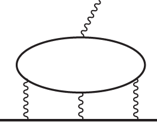
\includegraphics[width=0.20\textwidth]{AoHaKiNi12fig3d}}

Kinoshita correctly included external photon vertex insertions and
$\partial/\partial q$ derivatives into the electron line, but omitted the
electron loop derivatives.

\item[2019-06-04 Gerry Gabrielse]
The effects due to the finite radius of a Penning trap in which
the magnetic moment is measured are discussed in the 75-page
Lowell S. Brown and \HREF{https://www.physics.northwestern.edu/people/faculty/core-faculty/gerald-gabrielse.html}
{Gerald Gabrielse} 1986 paper\rf{BroGab86}
{\em Geonium theory: {Physics} of a single electron or ion in a {Penning} trap}.
At the end of section VII they say ``We conclude that the radiative
level shifts in geonium are certainly negligible.'' The also discuss
the effects of cylindrical cavity Green's function, find them negligible
as well, and much, much more. One deserves a Ph.D. just for being able to
get through this paper.

But, in the light of the increased experimental accuracies since 1986
some these claims might have to be reexamined.

As far as the QED $(g-2)$ calculation is concerned, I imagine one would
need to recompute the Schwinger $\alpha/2\pi$ with the photon (and
electron?) Green's function for a finite cylindrical container. This is a
much harder calculation, as instead of infinite Lorentz invariant free
space, one has to use the translation-symmetry broken photon Green's
function (photon propagator), with Dirichlet boundary conditions,
something like their frequency domain cylindrical Green's function
eq.~(8.25), expanded in terms of radial Bessel functions. All the magic
of usual Feynman integrals is gone; a job for a very good mathematical
physicist. They probably do not raise any such any more...

\item[2019-06-05 Predrag]
As an amusing curiosity / coincidence, today in our online plumbers'
meeting we discussed Burak's current work on ``Bohmian'' walking
droplets\rf{BudFle18}, an analysis of the ongoing IST Austria
experiments. The experiment is done in a shallow cylindrical dish, 8cm in
diameter, conical bottom with $1^o$ (!) slope. The equations are 2D
shallow wave approximation PDEs for the surface, coupled to a point-like
bouncing droplet, see sect.~III of the above reference. Currently Burak
plans to discretize his calculation on a grid, though eventually he might
try to use a radial Bessel function eigenmodes for his cell. DNS fluid
dynamicists do not use them, as they do not diagonalize Laplacians (not
sure - this statement looks wrong to me) and there are no fast numerical
Bessel transforms.

One person who could do Gabrielse calculation is der menschliche Panzer
Andreas Wirzba\rf{Wirzba99}. He will not listen to me, but Gabrielse
might persuade him.







%Thomai(female version of Thomas), James girlfriend, is from
%Tasos. Adanan, originally from Pakistan, teaches the QCD course.
%Nita Schubert is a nuclear chemist. he daughter, Dana (about 12 when I
%was in Morelia)
%was a pole bearer in the class graduation - she is the first in her year.

\end{description}
